
Unsere grundlegende Idee zur ROV-Analyse war folgende: Erst wollten wir das als munitionsbelastete gekennzeichnete Gebiet mithilfe 
des Multibeams grob kartieren und dabei 
interessante bzw. auffällige Stellen finden. Daraufhin wollten wir diese mit unserem ROV antauchen, um mit unser Kamera eine genauere Bestimmung durchführen zu können. 
Dieses Vorgehen konnten wir auch so zum Großteil durchführen.
Die genauer zu bestimmenden Stellen haben wir mit unserem eigenen ROV (Remotely Operated Vehicle), einer Art Tauchroboter, angetaucht. 
\subsubsection{Technische Beschreibung}
Dieser entstand vor drei Jahren in unsere Forschungsgruppe aus einem Bausatz der Firma BlueRobotics und trägt die Bezeichnung \emph{BlueROV 2}.
Der Tauchrobter lässt sich mithilfe eines Laptops und eines Controllers über ein langes Kabel (auch Tether genannt) frei in alle Richtungen in der Wassersäule bewegen.\\
Das ROV von BlueRobotics besteht aus zwei runden Druckgehäusen eines für den Lithium-Ionen Akku, das andere für die Steuerungselektonik und die Kamera.
Vor jedem Tauchgang müssen diese Druckgehäuse mithilfe einer Vakuumpumpe auf ihre Dichtigkeit überprüft werden. 
\begin{figure}[htb!]
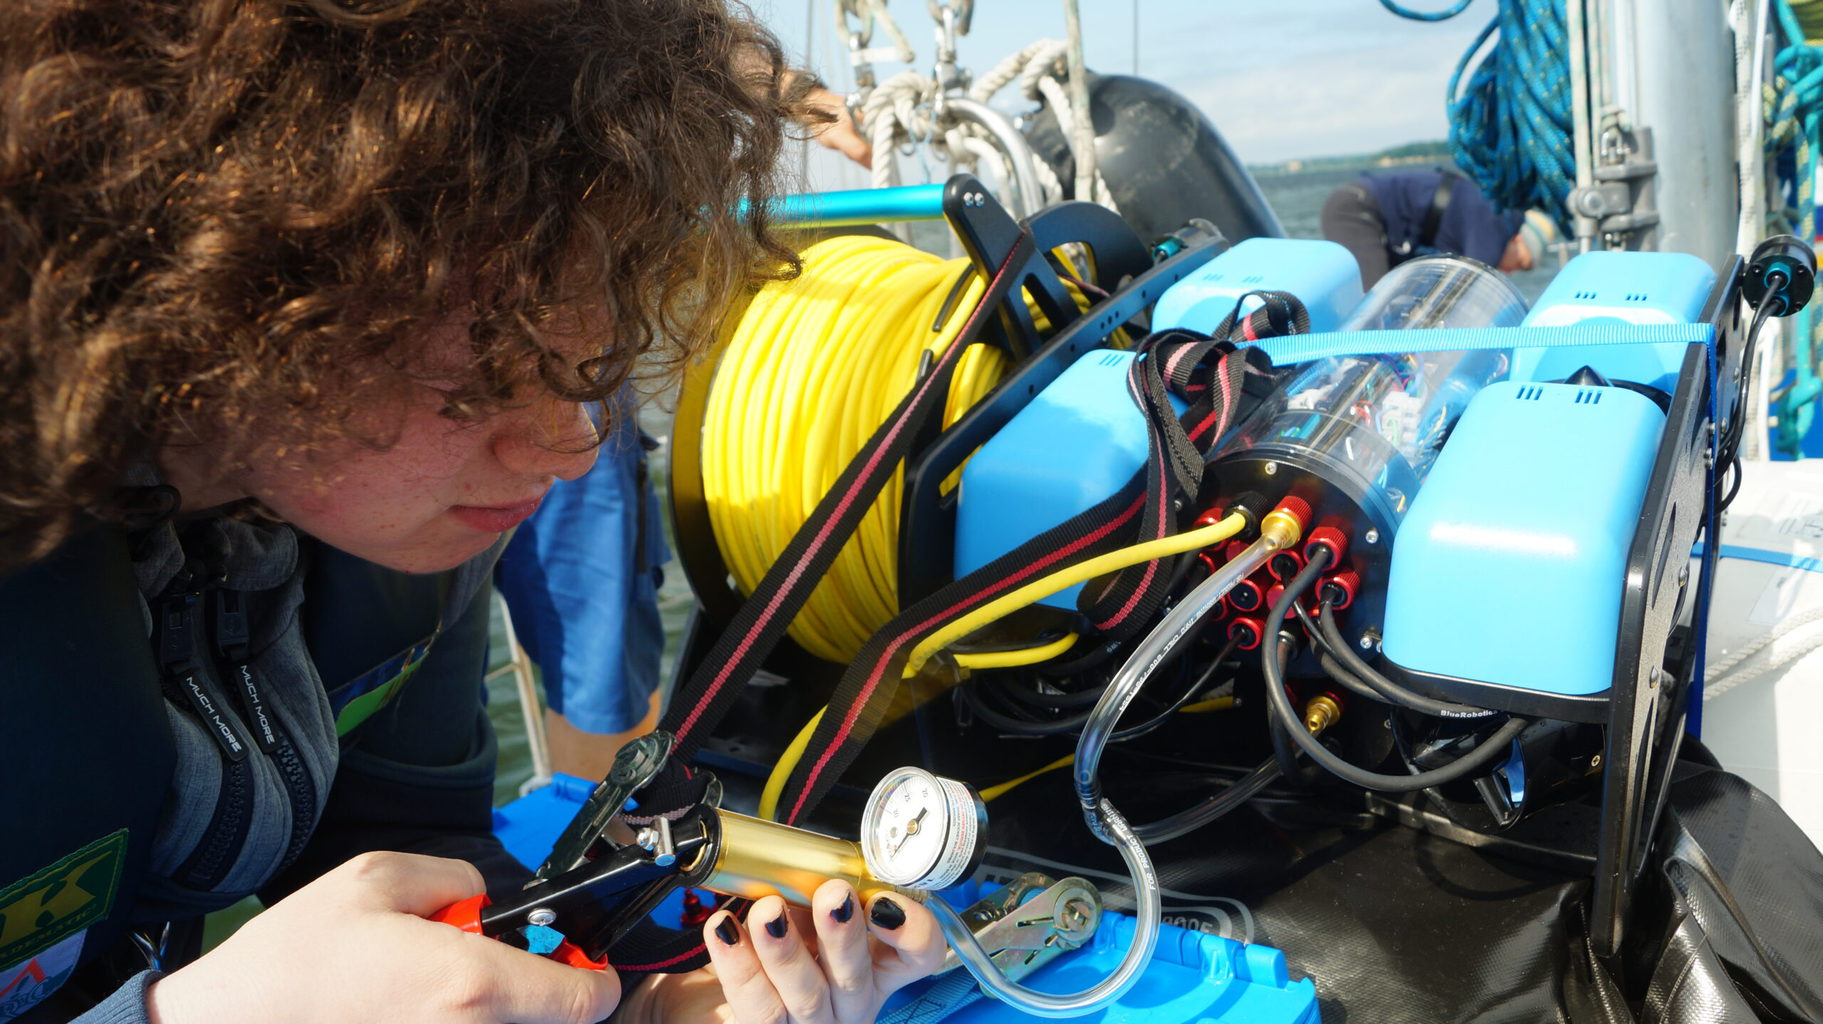
\includegraphics[height=\textheight,%
                   width=\textwidth,%
                   keepaspectratio]{Bilder/ROV/Druckpruefung.jpg}
\caption{Unterdruckprüfung vor der ROV-Fahrt}
\end{figure}
Anschließend wird das ROV mithilfe des Tethers an den Laptop angeschlossen werden, auf dem sich die Steuerungssoftware befindet.
\subsubsection{Operating auf der Aldebaran}
Der ROV wird optimalerweise 
von vier Personen bedient, da zwei Personen die Tetherspule bedienen müssen, man einen Navigator benötigt, da die Orientierung unter Wasser in einem fremdem Gebiet sehr anspruchsvoll ist und das ROV von einem Piloten gesteuert werden muss.
Somit beansprucht das ROV-Fahren unser gesamtes Forschungsteam und kann keine anderen Aufgaben, wie das Positionshalten des Forschungsschiffes o.ä. übernehmen. Deshalb ist das ROV-fahren für die gesamte Crew nicht nur zeitlich durchaus herausfordernd.
Aus diesem Grund war es besonders wichtig, gezielte Stellen ausfindig zu machen, an denen wir mit dem ROV abtauchen wollten und nicht nur blind im Meeresboden rumstochern.
\\

Um die Abläufe des ROV-tauchens richtig einzuspielen und den ROV auf der Aldebaran zu testen, haben wir am Sonntagabend einen Testtauchgang im Hafen durchgeführt. 
Hierbei ist uns schon die schlechte Sicht in der Ostee aufgefallen, die uns später noch einige Schwierigkeiten machen sollte.
\begin{figure}[htb]
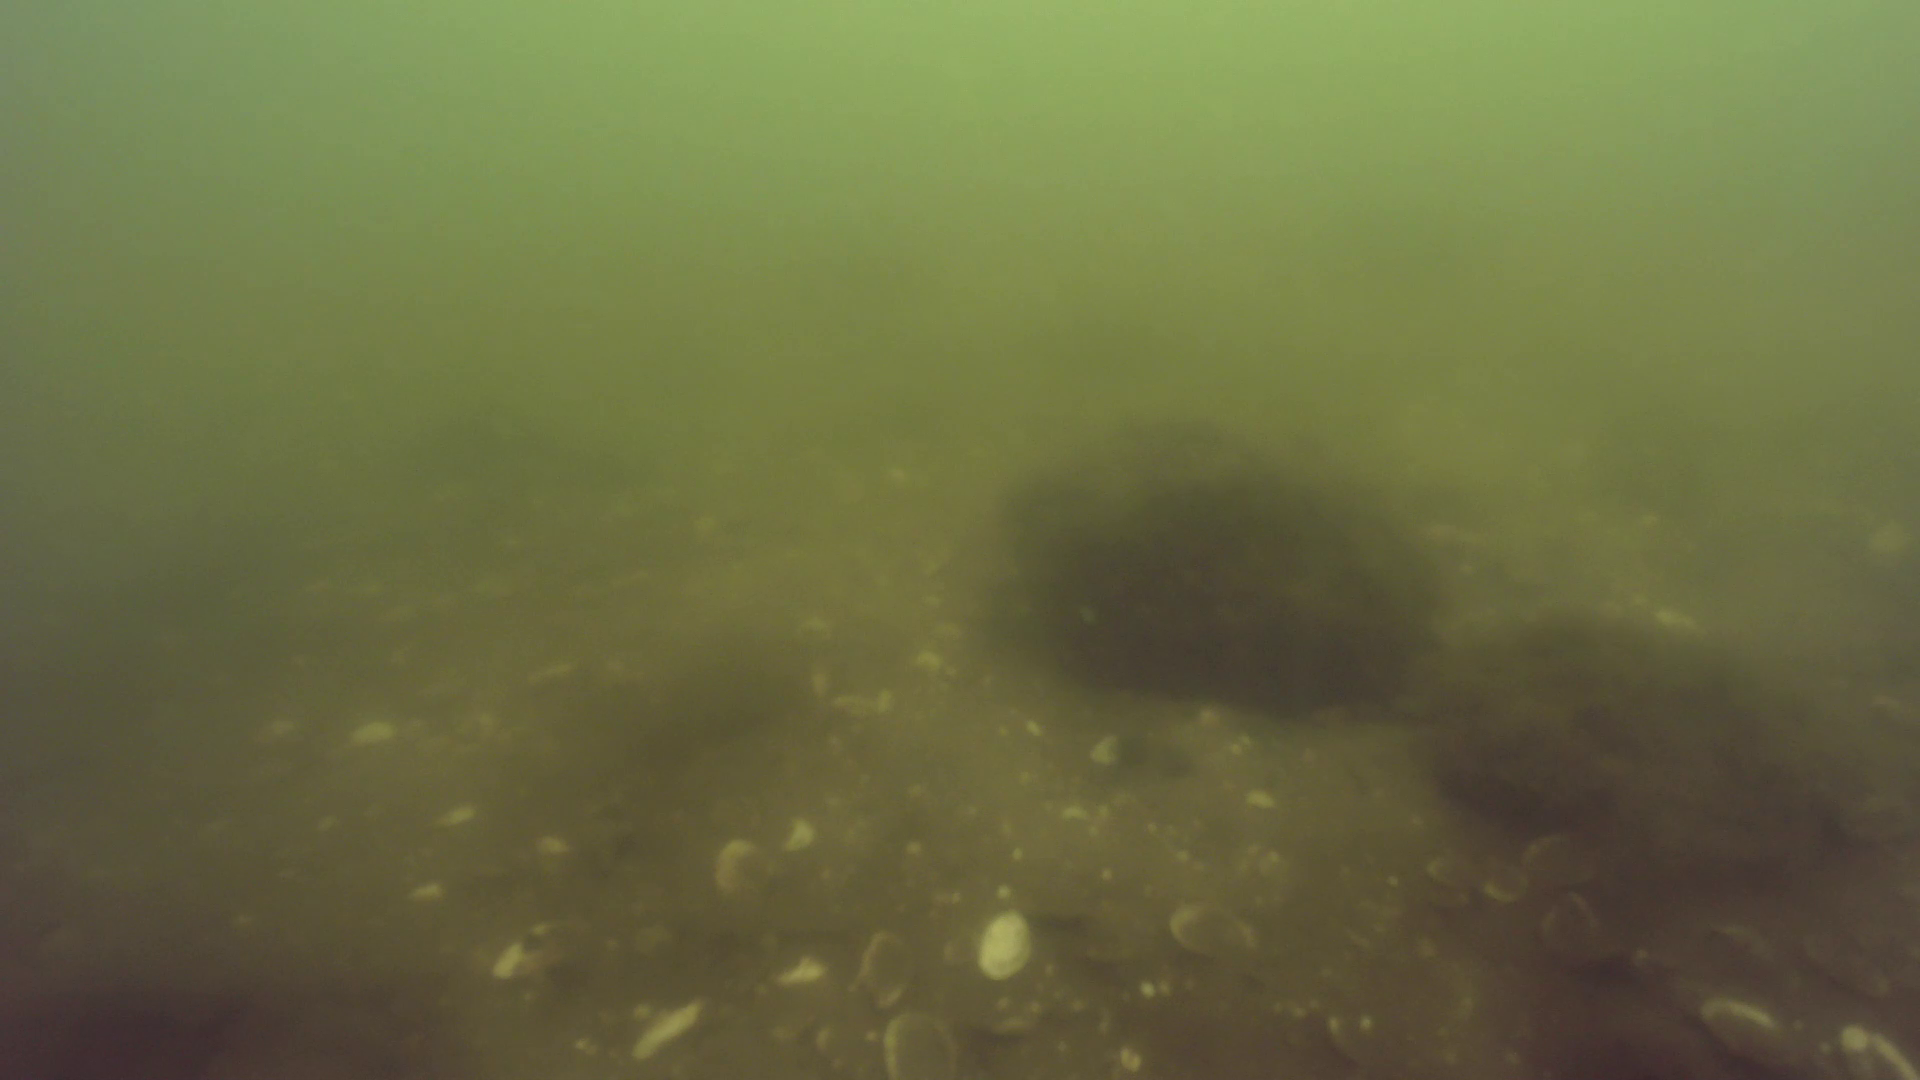
\includegraphics[height=\textheight,%
                   width=\textwidth,%
                   keepaspectratio]{Bilder/ROV/Steine.png}
\caption{Schlechte Unterwassersicht vor Lauerbach}
\end{figure}
\\

Insgesamt haben wir für unsere Forschung auf der Aldebaran an drei unterschiedlichen Stellen insgesamt fünf ROV Tauchgänge durchgeführt.
%Einfügen Karte mit Tauchstellen des ROV mit Objekten auf dem Multibeam
\subsubsection{Schwierigkeiten}
Während dieser Tauchgänge und bei deren Vorbereitung hatten wir einige unerwartete Schwierigkeiten.\\
Da die Aldebaran ein verhältnismäßig kleines Schiff für ein Forschungsschiff ist, hat sie zwar den Vorteil dass sie gerade durch das einklappbares Schwert einen sehr geringen Tiefgang von 80 cm hat, was uns die Forschung in diesem Gebiet erst ermöglicht hat.
Andererseits ist sie deshalb auch anfällig gegenüber Wind und Wetter, auch deshalb war das Arbeiten an Deck bei den zeitweise aufgetretenen Windstärken von vier bis fünf nicht immer einfach.\\
Dies hat sich sowohl bei der Vorbereitung des ROVs gezeigt als auch bei den Tauchgängen. Ein Problem war beispielsweise das Schwojen des Bootes am Anker.
Die Navigation und die Orientierung unter Wasser mit dem ROV war mit Abstand die größte Herausforderung, da die einzige Möglichkeit sich zu orientieren der eingebauter Kompass ist.
Unser ROV besitzt aufgrund seiner Größe kein USBL (Ultra Short Baseline) - System, wodurch die genaue Position des ROVs erst beim Auftauchen bekannt wird.
Eine durch das Multibeam angezeigte genaue Position haben wir angetaucht, indem wir diese über die Position des Schiffes angepeilt und versucht haben, bei Anfahrt durch den ROV diesen auf dem exakten Kompasskurs zu halten.
Durch das o.g. Schwojen ist die Fehlerquote hierbei schnell größer als die Sichtweite in der Ostsee. \\ Zusätzlich wurde das ROV 
durch die geringe Tauchtiefe von ca. 5m von den Wellendynamik und windinduzierter Strömung erfasst und im Kurs beeinflusst. 
Da wir selbst das ROV bisher lediglich auf Binnengewässern operiert haben, mussten wir zwangsläufig in vitro Erfahrungen mit dem ROV im Meereseinsatz sammeln, was die Trefferquote beim Anfahren interessanter Punkte zugegebenermaßen weiter verschlechterte. So spielte eine gute Portion Glück mit herein, was das Finden des angepeilten Objektes anging.\\
Trotz der Schwierigkeiten haben wir einige interessante Objekte mithilfe der optischen Kamera untersuchen können.\\


